

\documentclass{beamer}
 
\usepackage[utf8]{inputenc}
 \usetheme{Madrid}
 \usecolortheme{beaver}
 \usefonttheme{structuresmallcapsserif}
 \usepackage{listings}
%Information to be included in the title page:


\title[Overview] %optional
{Devices}

\subtitle{An Overview}

\author[Dr. Joseph Kehoe] % (optional, for multiple authors)
{Joseph Kehoe\inst{1}}

\institute[IT Carlow] % (optional)
{
	\inst{1}%
	Department of Computing and Networking\\
	Institute of Technology Carlow
}

\date[ITC 2017] % (optional)
{CDD101, 2017}

\logo{
\includegraphics[height=1.5cm]{../../itcarlowlogo.png}}




 
 \AtBeginSection[]
 {
 	\begin{frame}
 		\frametitle{Table of Contents}
 		\tableofcontents[currentsection]
 	\end{frame}
 }
 
 
 
\begin{document}
 
\frame{\titlepage}
 
 
 
 \begin{frame}
 	\frametitle{Table of Contents}
 	\tableofcontents
 \end{frame}
 
 
 \section{Some Definitions}
\begin{frame}
\frametitle{Definitions}
\begin{description}
	\item[Device] a thing made or adapted for a particular purpose, especially a piece of mechanical or electronic equipment.
	\item[Device] a piece of equipment or a mechanism designed to serve a special purpose or perform a special function.
	\item[IoT] the interconnection via the Internet of computing devices embedded in everyday objects, enabling them to send and receive data.
\end{description}

\end{frame}

\begin{frame}
	\frametitle{Growth}
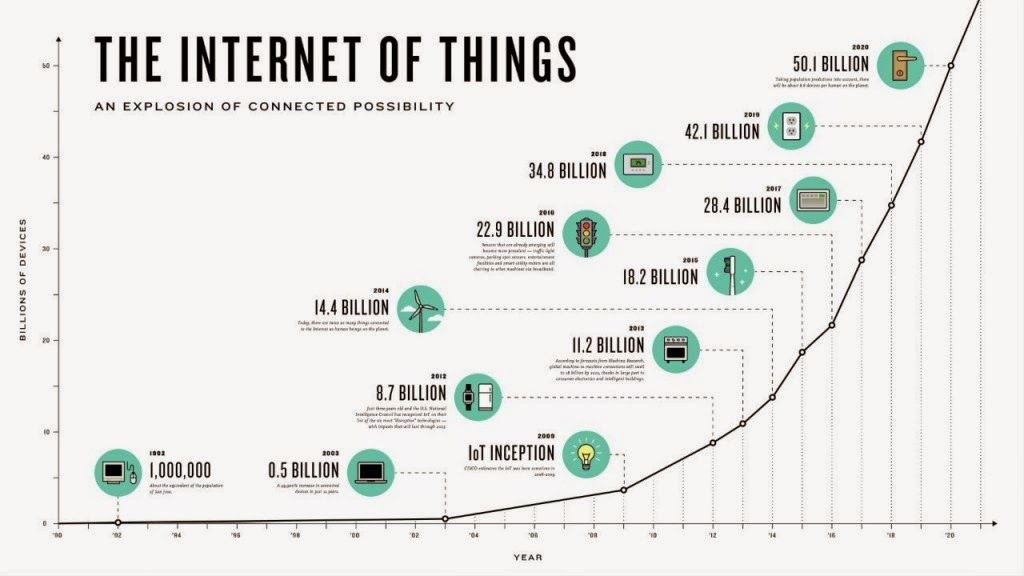
\includegraphics[height=6cm]{growth.jpg}
	
\end{frame}

 \section{Some Examples}
\begin{frame}
	\frametitle{Examples}
	
     \begin{itemize}
     	\item Cars
     	\item Kitchen Appliances
     	\item Medical Equipmen
     	\item Military Equipment
     	\item Wearables
     \end{itemize}
     
\begin{itemize}
	\item How many devices are you carrying at the moment?
     
     \item Devices are becomming programmable - this is a huge change!
     
     \item Devices can include Sensors and Actuators - this gives them unique advantages or GP Computers
\end{itemize}
\end{frame}


\begin{frame}
	\frametitle{Growth}
	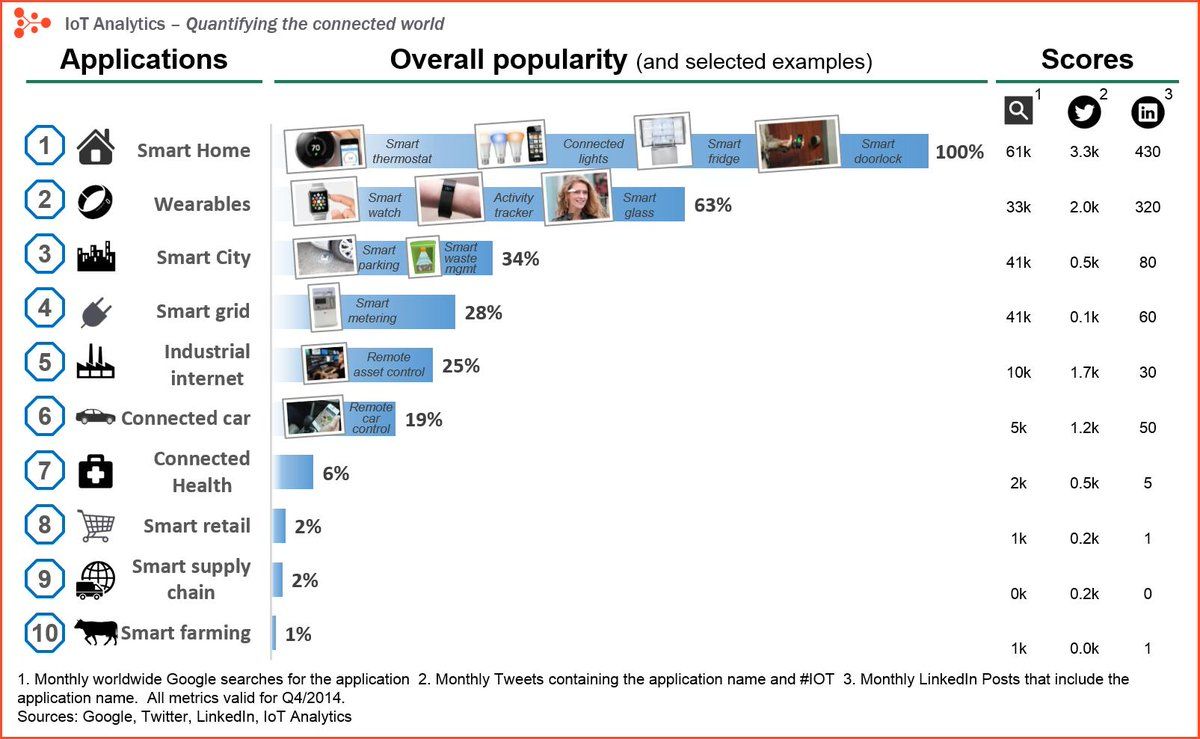
\includegraphics[height=6cm]{deviceApps.jpg}
	
\end{frame}



  \section{Sensors and Actuators}
  \begin{frame}
  	\frametitle{Sensors and Actuators}
\begin{description}
	\item[Sensor]A device which detects or measures a physical property and records, indicates, or otherwise responds to it
	\item[Actuator] A component that is responsible for moving or controlling a mechanism or system; in simple terms, it is a "mover". An actuator requires a control signal and a source of energy. There are five main types of actuators – hydraulic, pneumatic, electrical, Thermal or Magnetic and Mechanical.
\end{description}


  \end{frame}
 \begin{frame}
 	\frametitle{Growth}
 	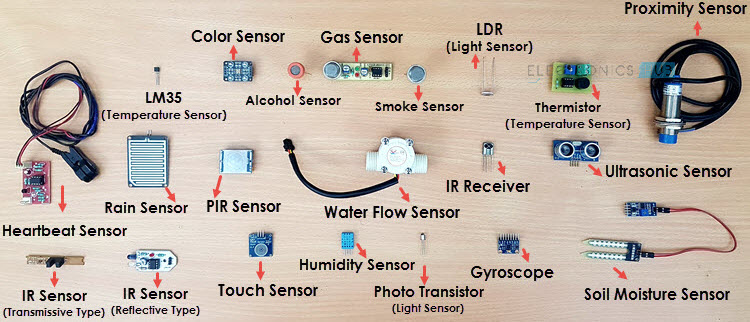
\includegraphics[height=5cm]{Types-of-Sensors.jpg}
 	
 \end{frame}
  
   \section{General Architecture}
   \begin{frame}
   	\frametitle{General Architecture}
Each type of device can have a unique architecture. The differ from GP Computing architecture in:
\begin{itemize}
	\item Power Constraints
	\item Speed Constraints
	\item Space Constraints
\end{itemize}

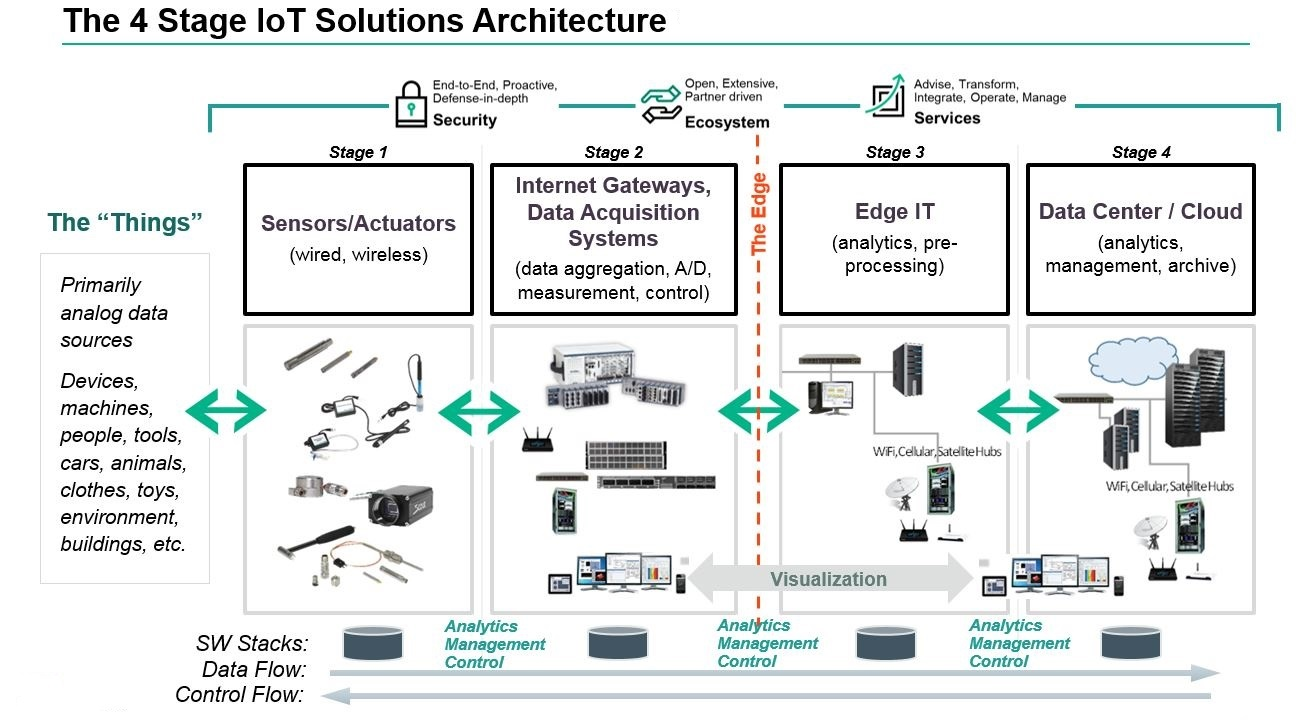
\includegraphics[height=4cm]{iotArchitecture.jpg}

   \end{frame}
     \section{Issues}
     \begin{frame}
     	\frametitle{Issues}
     \begin{itemize}
     	\item We are restricted in how we program a device
     	\item UX/UI design must be completely rethought
     	\item How do we stay connected?
     	\item Security and privacy issues
     \end{itemize}	
     \end{frame}   

    

        
\end{document}

